
\documentclass[conference]{IEEEtran}

\usepackage{booktabs}       % professional-quality tables
\usepackage{color}
\usepackage{graphicx}
\usepackage{subfigure}
\usepackage{comment}
\usepackage[fleqn]{amsmath}
\usepackage{multirow}
\usepackage{comment}

\ifCLASSINFOpdf
 
\else

\fi

\hyphenation{op-tical net-works semi-conduc-tor}

\newcommand{\tabincell}[2]{\begin{tabular}{@{}#1@{}}#2\end{tabular}}

\begin{document}
 
\title{Plankton Classification with Hybrid Convolutional Neural Network}


\author{\IEEEauthorblockN{Jinna Cui}
\IEEEauthorblockA{College of Information Science and Engineering\\
Ocean University of China\\
Qingdao 266100, China\\
Email: Jinna\_ouc@163.com}}


\maketitle


\begin{abstract}
Plankton are the foundation of marine ecosystem marine food chain. Plankton are of great value in environmental protection and fishing industries, as a result, the research on plankton plays an essential role in ecosystem balance and economic development. Plankton classification is an important part of plankton research. However, the huge amount and tiny volume of plankton make plankton classification extremely difficult. In this paper, the database we use is a large scale database named WHOI-Plankton, it contains over 3 million images, labeled into 103 classes. Traditional method of plankton classification on this database is time consuming and the effect is poor. In contrast, deep neural network can get great result. The approach of plankton classification we presented is based on convolutional neural network model. Our network structure is designed into a inverse pyramid shape in fully connect layer\cite{accv2016Dai} to combine information from three channels. In order to get higher classification accuracy, we try to smooth images and remove noises by lowpass filtering and abstract images details and edges by highpass filtering. Gaussian filtering can get good filter effect and reduce ringing effect, so we chose Gaussian lowpass filtering and Gaussian highpass filtering. With this method, neural network can abstract more higher-level features and get more information from training images, in this way, we can get better result in plankton classification.  In this way, we can integrate these 3 classes features well and get higher accuracy. The result of experiments on WHOI shows that our neural network achieves higher accuracy than original convolutional neural network.
\end{abstract}
\IEEEpeerreviewmaketitle


\section{Introduction}

WHOI-Plankton is publicly released by Woods Hole Oceanographic Institution\cite{DBLP:journals/corr/OrensteinBPS15}. They collected these images for 8 years, and labelled them into 103 classes, some images of WHOI-Plankton database is showed in Fig.1. We picked images collected in 2014 out as testing data, and the others are training data.  In this paper, we set AlexNet\cite{krizhevsky2012imagenet} as a baseline and trained WHOI-Plankton on it. AlexNet is a typical and efficient convolutional neural network widely used in images classification.

\begin{figure}[!ht]
\centering
\subfigure{
  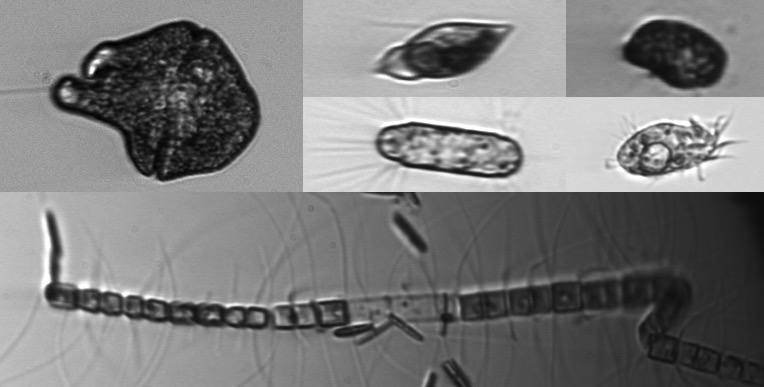
\includegraphics[width=0.5\linewidth]{samples.jpg}}
  \hspace{0.05in}
  \caption{Samples of WHOI-Plankton}
\end{figure}

\section{Proposed Method}
In order to enhance the capability of neural network\cite{DNN}  abstracting features from plankton images, we proposed a three-sub networks based on AlexNet. These three sub networks  share one label and output error but they has their own input. The inputs of each network are as follows: original images, GHPF(Gaussian Highpass Filter) images, GLPF(Gaussian Lowpass Filter) images. Example images are showed in Fig.2. 
 \newline
 \newline
 
\begin{figure}[!ht]
\centering
\subfigure[original image]{
  \label{fig:a}
  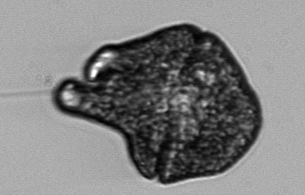
\includegraphics[width=0.45\linewidth]{original.png}}
  \hspace{0.15in}
\subfigure[GHPF image]{
  \label{fig:b}
  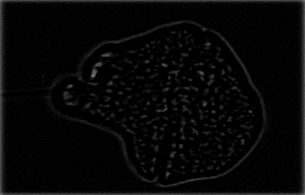
\includegraphics[width=0.45\linewidth]{GHPF.png}}
  \hspace{0.15in}
  \subfigure[GLPF image]{
  \label{fig:c}
  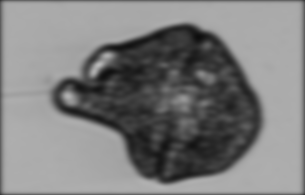
\includegraphics[width=0.45\linewidth]{GLPF.png}}
  \hspace{0.15in}
  \caption{Samples of processed images}
\end{figure}


The architecture of our model used in the experiment. Convolution layer of every network contains 5 convolution layers and two pooling layer followed the first two convolution layer. The pooling method is 3\begin{math} \times \end{math}3 max pooling. After convolution, the full connect layers are designed a inverse pyramid shape to combine different features. 



\begin{figure*}[!ht]
\centering
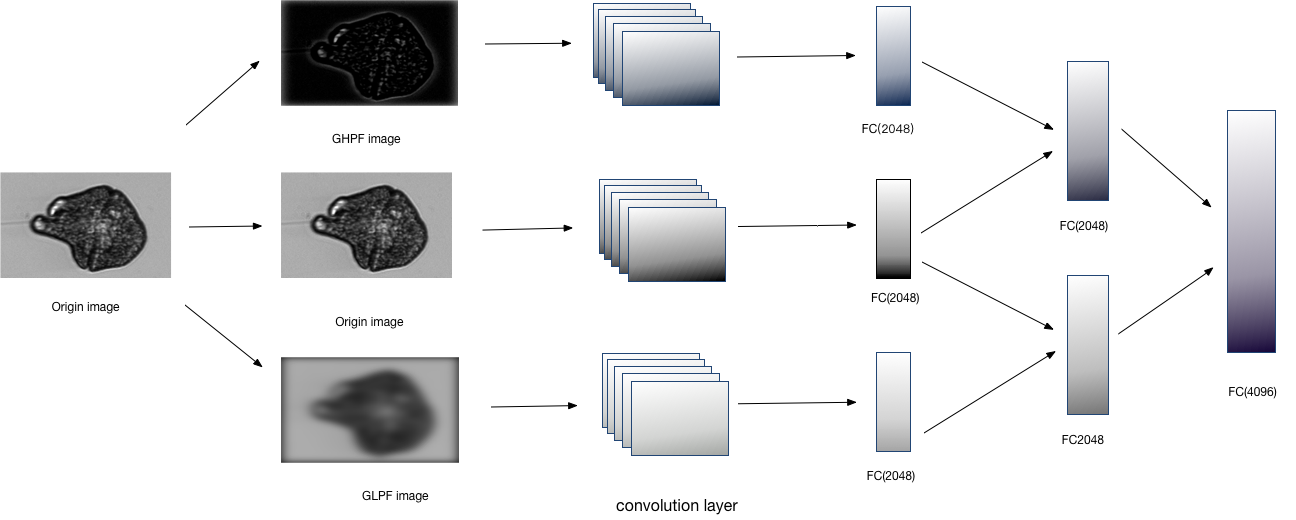
\includegraphics[width=0.85\textwidth]{network}
\caption{Structure of our neural network.}
\label{fig:network}
\end{figure*}


\newpage
\section{Experiments}
% table
\begin{table}[!ht]
  \caption{Accuracy of Plankton Classification}
  \centering
  \begin{tabular}{lllll}
    \toprule
    \cmidrule{1-3}
    database     &model       &accuracy  \\
    \midrule
    full & AlexNet trained on original images   & 0.9358 \\ \hline
    full & AlexNet trained on 3-channels images   &0.9421   \\
    \bottomrule
  \end{tabular}
\end{table}

%neural network archiecture



\section{Conclusion}
We presented a hybrid neural network to increase the accuracy of plankton classification and processed images by filter. With this method, we got higher accuracy than original convolutional neural network. 
\bibliographystyle{IEEEtran}
\bibliography{Oceans17}


% that's all folks
\end{document}


